\section{Definició de models}
Per la predicció de la variable objectiu (\textit{Status}) s'han realitzat 3 tipus diferents de models: un K-Nearest Neighbors (KNN), un Arbre de Decisió (Decision Tree) i un Support Vector Machine (SVM). 

En primer lloc, cal mencionar que tots aquests models treballen amb dades numèriques, de manera que requereixen que les dades categòriques hagin estat codificades. No obstant, en la implementació que s'ha fet, es contempla el cas en què les variables categòriques no han estat codificades i llavors el model prediu només amb les variables categòriques. Això ens permet poder fer proves amb i sense codificar les dades, ja que en certs models i datasets potser s'obté millor rendiment obviant les variables numèriques en la predicció.

Per cada un dels models, es definiran uns paràmetres generals fixes (els que generalment venen per defecte en els predictors de \texttt{scikit-learn}) i es provaran totes les possibles combinacions de modificacions al dataset (codificar o no, eliminar o no outliers, escalar variables o no, balancejar classes amb un mètode o amb un altre, etc.) mitjançant la funció \texttt{find\_best\_dataset()}. En cada una d'aquestes combinacions s'entrena el model i es fa la predicció, obtenint els resultats. El dataset (combinació de modificacions al dataset inicial) que aconsegueixi millors resultats (predient en el test) s'establirà com el ``millor dataset pels models d'aquell tipus''.

Una vegada determinat el millor dataset per cada tipus de model, es provaran moltes combinacions de paràmetres en les funcions \texttt{X\_prediction()} (on \texttt{X} serà \texttt{knn}, \texttt{dt} o \texttt{svm}, depenent del model) mitjançant cross validation en la partició de train. Els que donin millors resultats de mitjana en la validació s'utilitzaran per predir en el test i es determinarà com el ``model definitiu d'aquell tipus'' (ja que s'haurà entrenat amb un dataset específic per al model en concret i s'hauran trobat els paràmetres que rendeixen millor).

Evidentment, les proves es podrien fer directament sempre al test (no a la partició de validació) i també provar una major quantitat de paràmetres i combinacions de datasets dels que es provaran. No obstant, es considera que una de les parts fonamentals d'aquest projecte consisteix en saber filtrar què pot funcionar i què no, en comptes de provar-ho tot a la força bruta. És a dir, encara que els paràmetres que s'escullin en el validation no acabin sent els millors pel test (ja que poden estar donant mètriques més altes en el validation degut a overfitting), no és una solució eficient (ni en termes de computació, ni de temps, ni de escalabilitat, etc.) provar tots aquests paràmetres en el test directament. A més, les particions de validació estan fetes precisament per ajudar a escollir paràmetres.

Una vegada mencionat això, quan ja es tinguin els 3 ``models definitius'', es compararan els resultats per escollir el millor dels 3 models i procedir al seu anàlisi més exhaustiu, model card, etc.

Totes aquestes proves o execucions es realitzaran amb la llavor (seed o random\_state) amb valor 42 arbitràriament per una millor reproductibilitat. És evident que s'obtindrien millors resultats realitzant l'experiment amb múltiples llavors i escollint els paràmetres que més es repetissin en les diferents execucions (per així reduir el factor aleatori), però cada una d'aquestes execucions té una durada aproximada de 20 minuts, de manera que no és viable perdre-hi tant de temps. No obstant, si s'haguessin d'implementar aquests models en un cas real, seria molt important afegir més execucions amb llavors diferents per poder tenir resultats més robustos al factor aleatori.

A continuació es detallen els diferents tipus de models, els paràmetres provats, el conjunt de modificacions del dataset adient per cada un, les mètriques utilitzades, etc.

\subsection{K-Nearest Neighbors (KNN)}

\subsubsection{Motivació}
El nostre dataset conté dades relacionades amb pacients amb cirrosi hepàtica, on l'objectiu principal és predir l'estat del pacient (variable \textit{Status}). L'algorisme \textit{K-Nearest Neighbors} (KNN) es presenta com una elecció adequada per aquesta tasca per diverses raons.

En primer lloc, KNN és un algorisme basat en instàncies, el que significa que fa prediccions basant-se en la proximitat i similitud de les mostres en l'espai de característiques. Això és particularment útil en el nostre cas, on les característiques dels pacients com l'edat, sexe, indicadors bioquímics i la resposta al tractament poden influir directament en el seu estat de salut. La capacitat de KNN per capturar aquestes relacions espacials i fer prediccions sense la necessitat de que hi hagi patrons explícits el fa un bon candidat per conjunts de dades amb relacions complexes i no lineals entre les característiques i la variable objectiu.

A més, la naturalesa intuïtiva i la facilitat d'interpretació de KNN són avantatges significatius quan es tracta de dades mèdiques. La possibilitat de explicar les prediccions en termes de "pacients semblants" (\textit{Nearest Neighbors}) pot ser molt valuosa en l'àmbit mèdic, on la comprensió i la confiança en el model són també de gran importància.

\subsubsection{Mètriques}
Per l'avaluació del model, s'ha utilitzat la mètrica de \textit{f1-score-weighted}, tal i com s'ha dit que es faria en tots els models (inclosos els de imputació explicats en apartats anteriors). Aquesta mètrica és calcula fent la mitjana harmònica entre la \textit{precision} i el \textit{recall}, penalitzant els valors extrems (calen valors bons tant de \textit{precision} com de \textit{recall} per tal de tenir un bon \textit{f1}). La mitjana de valors de totes les prediccions es fa ponderada (\textit{weighted}), de manera que a cada classe se li dona una importància proporcional a les seves aparicions. D'aquesta manera, es puntua millor que s'aconsegueixi classificar correctament la classe majoritària (on s'haurà de fer més prediccions). 

Si en un altre experiment es desitgés predir donar molta importància la classe minoritària (en aquest cas ``LiverTransplant'', que no és tant rellevant en aquest estudi com ``Alive'' o ``Dead'') es podrien utilitzar altres mètriques que ho tinguessin més en consideració.

\subsubsection{Hiperparàmetres}
L'únic hiperparàmetre que s'ha modificat és la \textit{k} (\texttt{n\_neighbors} en la implementació de \texttt{scikit-learn}), que indica el nombre de veïns més propers que es consideren a l'hora de fer la predicció. Els valors que s'han provat són 1, 2, 3, 5, 10, 15, 20 ,25 i 50.

\subsubsection{Millor conjunt de dades}
Per trobar el conjunt de dades que proporciona un millor rendiment a aquest model, s'han fixat els hiperparàmetres a $k = 3$ i s'ha executat la funció \texttt{find\_best\_dataset()}. Després que es provin totes les combinacions possibles de modificacions al dataset inicial (un total de 64 combinacions), la que ha obtingut millors resultats de \textit{f1-score-weighted} en el test és la següent:
\begin{itemize}
	\item No eliminar outliers.
	\item Eliminar les files amb més de 9 NaNs.
	\item Escalar les variables numèriques amb \textit{MinMax}.
	\item Imputar variables numèriques amb KNN Imputer (amb $k = 15$) i les categòriques amb Random Forest Classifier (amb el criteri `gini'). Els resultats de la imputació (calculats tal i com s'ha explicat en l'apartat \ref{subsec:missings}) han estat de 0,3808 de mitjana entre la puntuació $R^2$ de les numèriques i \textit{f1-score-weighted} de les categòriques.
	\item No codificar les variables categòriques.
	\item No balancejar les classes de la variable objectiu.
\end{itemize}

Amb aquestes modificacions i els paràmetres fixes que s'han mencionat, s'ha aconseguit un resultat de 0,7838 de \textit{f1-score-weighted} en el conjunt de prova (test), que es pot considerar un resultat bastant bo. La partició de train conté 277 mostres i la de test 50. A partir d'aquí s'ha considerat que aquests són els millors conjunts de dades per els models KNN, i el següent pas serà trobar els millors paràmetres per el model en aquest dataset.

\subsubsection{Millors hiperparàmetres pel dataset escollit}
Una vegada determinat el millor dataset per els models KNN, cal provar quins són els millors paràmetres. Això es fa mitjançant la funció \texttt{run\_experiment()} que cridarà a \texttt{knn\_prediction()}. En aquesta segona funció s'implementa cross validation amb 5 \textit{folds} per cada possible combinació de paràmetres. Una vegada s'hagin provat tots els paràmetres, la combinació de paràmetres que tingui un millor \textit{f1-score-weighted} de mitjana en la partició de validació (és a dir, el que obtingui una millor puntuació en la validació creuada) es determinarà com la millor per el model KNN i s'executarà la predicció en el test.

Una vagada s'ha fet la l'execució, s'ha obtingut que el millor paràmetre és $k = 25$, amb una puntuació en la partició de validació de 0,6287.

\subsubsection{Resultats}
Amb el dataset escollit i els millors hiperparàmetres triats, la predicció en el conjunt ha obtingut les mètriques que es poden veure en la taula \ref{tab:knn-test}

\begin{table}[H]
\centering
\begin{tabular}{l|l}
\hline
\textbf{Metric} & \textbf{Value} \\
\hline
accuracy & 0.76 \\
f1-micro & 0.76 \\
f1-macro & 0.5228251507321274 \\
f1-weighted & 0.736537677002583 \\
precision-micro & 0.76 \\
precision-macro & 0.5075757575757576 \\
precision-weighted & 0.7145454545454545 \\
recall-micro & 0.76 \\
recall-macro & 0.539072039072039 \\
recall-weighted & 0.76 \\
\hline
\end{tabular}
\caption{Mètriques obtingudes en l'execució de KNN en la partició de test amb el millor dataset pel model i els millors paràmetres ($k = 25$).}
\label{tab:knn-test}
\end{table}

Si ens fixem en la mètrica que hem escollit (\textit{f1-score-weighted}), podem veure que s'ha obtingut un valor de 0,7365, que està bastant bé. Aquest valor és més alt del que s'ha obtingut en la partició de validació. Això segurament succeeix per un factor aleatori.

Pel que fa a les prediccions, en la figura \ref{fig:knn-cm} es pot veure la matriu de confusió d'aquest model en les prediccions del conjunt de test. Es pot apreciar que la majoria de prediccions són bones. No obstant, hi ha hagut 5 mostres `Alive' que s'han predit com a `Dead' i 4 mostres de `Dead' que s'han predit com `Alive', de manera que el model no és perfecte i en alguns casos s'equivoca. Pel que fa a la classe `LiverTransplant', hi ha molt poques mostres (només 3) i el model no ha sigut capaç de predir-les correctament, ja que les ha predit com a `Alive'. Tot i això, cal considerar que realment els pacients que ha tingut un transplant de fetge (`LiverTransplant') han acabat sobrevivint... de manera que aquest error en la predicció és menys greu que els de les altres classes.

Per poder extreure més conclusions sobre les prediccions de `LiverTransplant' seria útil conèixer en quines condicions una persona pot acabar rebent un transplant de fetge. És a dir, el pacient ha de complir unes condicions de salut per tal de que es faci el transplant o simplement cal que s'aconsegueixi un donador? Això podria ajudar a determinar millor si és millor que els valors que nos s'han predit correctament de `LiverTransplant' es prediguin com a `Alive' o com a `Dead'.

\begin{figure}[H]
	\centering
	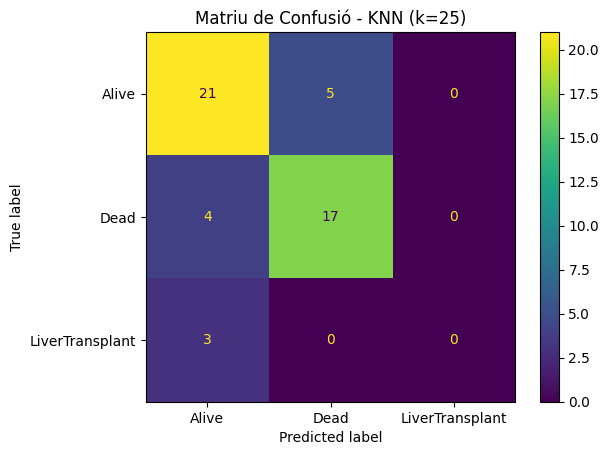
\includegraphics[width=0.85\linewidth]{img/knn-cm.png}
	\caption{Matriu de confusió de les prediccions del KNN (amb paràmetres $k = 25$) en el conjunt de test.}
	\label{fig:knn-cm}	
\end{figure}

Tot i el desbalanceig de classes, el model és aproximadament igual de bo predint la classe `Alive' (amb una proporció de $\dfrac{21}{26} \approx 0.8077$ prediccions correctes en aquesta classe) que la classe `Dead' (amb una proporció de $\dfrac{17}{21} \approx 0.8095$ prediccions correctes en aquesta classe).

%--------------------------------------------------------------------------
\subsection{Arbre de Decisió}

\subsubsection{Motivació}
El nostre dataset presenta dades complexes i diverses sobre pacients amb cirrosi hepàtica, on la tasca principal és predir l'estat del pacient (\textit{Status}). L'ús d'un arbre de decisió per a aquesta finalitat pot ser útil degut a que són models no lineals que poden capturar interaccions complexes entre les variables. Això és particularment útil en el nostre cas, ja que la condició dels pacients pot estar influenciada per una combinació de factors com ara l'edat, el sexe, els indicadors bioquímics, etc. . Un arbre de decisió pot dividir l'espai de les dades en subconjunts basats en aquestes característiques, facilitant la comprensió de com aquests factors interactuen i afecten el \textit{Status} del pacient.

\subsubsection{Mètriques}
De la mateixa manera que s'ha fet per al KNN, en l'avaluació del model s'ha utilitzat la mètrica de \textit{f1-score-weighted}. Aquesta mètrica és calcula fent la mitjana harmònica entre la \textit{precision} i el \textit{recall}, penalitzant els valors extrems (calen valors bons tant de \textit{precision} com de \textit{recall} per tal de tenir un bon \textit{f1}). La mitjana de valors de totes les prediccions es fa ponderada (\textit{weighted}), de manera que a cada classe se li dona una importància proporcional a les seves aparicions. D'aquesta manera, es puntua millor que s'aconsegueixi classificar correctament la classe majoritària (on s'haurà de fer més prediccions). 

Si en un altre experiment es desitgés predir donar molta importància la classe minoritària (en aquest cas ``LiverTransplant'', que no és tant rellevant en aquest estudi com ``Alive'' o ``Dead'') es podrien utilitzar altres mètriques que ho tinguessin més en consideració.

\subsubsection{Hiperparàmetres}
Pel que fa als hiperparàmetres de l'arbre de decisió, s'han modificat el criteri de decisió, la profunditat màxima, el nombre mínim de mostres per cada fulla i el nombre mínim de mostres per dividir un conjunt de l'arbre.

Els valors que es provaran per cada un dels paràmetres són els següents:
\begin{itemize}
	\item \textbf{Criteri}: `entropy' i `gini'.
	\item \textbf{Max\_depth}: None, 2, 3, 5, 10, 20, 50.
	\item \textbf{Min\_samples\_leaf}: 1, 2, 3, 5, 10, 20 ,50.
	\item \textbf{Min\_samples\_split}: 2, 3, 5, 10, 20, 50.
\end{itemize}

Totes les possibles combinacions d'aquests paràmetres es provaran mitjançant  Grid Search i cross validation per trobar els que millor rendiment aporten al model.

\subsubsection{Millor conjunt de dades}
Per trobar el conjunt de dades que proporciona un millor rendiment a aquest model, s'han fixat els següents hiperparàmetres:
\begin{itemize}
	\item \textbf{Criteri}: `entropy'.
	\item \textbf{Max\_depth}: None.
	\item \textbf{Min\_samples\_leaf}: 1.
	\item \textbf{Min\_samples\_split}: 2.
\end{itemize}

Amb aquests paràmetres fixats, s'ha executat la funció \texttt{find\_best\_dataset()}. Després que es provin totes les combinacions possibles de modificacions al dataset inicial (un total de 64 combinacions), la que ha obtingut millors resultats de \textit{f1-score-weighted} en el test és la següent:
\begin{itemize}
	\item No eliminar outliers.
	\item Eliminar les files amb més de 9 NaNs.
	\item No escalar les variables numèriques.
	\item Imputar variables numèriques amb Iterative Imputer (amb Lineal Regression com a estimador) i les categòriques amb Random Forest Classifier (amb el criteri `gini'). Els resultats de la imputació (calculats tal i com s'ha explicat en l'apartat \ref{subsec:missings}) han estat de 0,3581 de mitjana entre la puntuació $R^2$ de les numèriques i \textit{f1-score-weighted} de les categòriques.
	\item Codificar les variables categòriques amb \textit{Ordinal Encoding}.
	\item Balancejar les classes de la variabe objectiu mitjançant \textit{Oversampling}.
\end{itemize}

Amb aquestes modificacions i els paràmetres fixes que s'han mencionat, s'ha aconseguit un resultat de 0,7849 de \textit{f1-score-weighted} en el conjunt de prova, que es pot considerar un resultat bastant bo. La partició de train conté 441 mostres i la de test 50. A partir d'aquí s'ha considerat que aquests són els millors conjunts de dades per els models d'Arbre de Decisió, i el següent pas serà trobar els millors paràmetres per el model en aquest dataset.

\subsubsection{Millors hiperparàmetres pel dataset escollit}
Una vegada determinat el millor dataset per els models d'Arbre de Decisió, cal provar quins són els millors paràmetres. Això es fa mitjançant la funció \texttt{run\_experiment()} que cridarà a \texttt{dt\_prediction()}. En aquesta segona funció s'implementa cross validation amb 5 \textit{folds} per cada possible combinació de paràmetres. Una vegada s'hagin provat tots els paràmetres, la combinació de paràmetres que tingui un millor \textit{f1-score-weighted} de mitjana en la partició de validació (és a dir, el que obtingui una millor puntuació en la validació creuada) es determinarà com la millor per el model d'Arbre de Decisió i s'executarà la predicció en el test.

Una vagada s'ha fet la l'execució, s'ha obtingut que la millor combinació de paràmetres és la següent:
\begin{itemize}
	\item \textbf{Criteri}: `gini'.
	\item \textbf{Max\_depth}: None.
	\item \textbf{Min\_samples\_leaf}: 1.
	\item \textbf{Min\_samples\_split}: 2.
\end{itemize}

Amb aquests paràmetres s'ha obtingut una puntuació en la partició de validació de 0,8319.

\subsubsection{Resultats}
Amb el dataset escollit i els millors hiperparàmetres triats, la predicció en el conjunt ha obtingut les mètriques que es poden veure en la taula \ref{tab:dt-test}

\begin{table}[H]
\centering
\begin{tabular}{l|l}
\hline
\textbf{Metric} & \textbf{Value} \\
\hline
accuracy & 0.7 \\
f1-micro & 0.7 \\
f1-macro & 0.5724135182528296 \\
f1-weighted & 0.7096724055475849 \\
precision-micro & 0.7 \\
precision-macro & 0.5666666666666667 \\
precision-weighted & 0.722 \\
recall-micro & 0.7 \\
recall-macro & 0.5897435897435898 \\
recall-weighted & 0.7 \\
\hline
\end{tabular}
\caption{Mètriques de les prediccions de l'Arbre de Decisió (amb paràmetres \textit{criterion = `gini', max\_depth = None, min\_samples\_leaf = 1} i \textit{min\_samples\_split = 2}) en el conjunt de test.}
\label{tab:dt-test}
\end{table}

Si ens fixem en la mètrica que hem escollit (\textit{f1-score-weighted}), podem veure que s'ha obtingut un valor de 0,7097, que és un valor considerablement bo. A més, en aquest cas el valor sí que es menor a l'obtingut en la validació creuada, de manera que podem dir que segurament el nostre model té un lleuger overfitting en les dades del train. Tot i això, a l'hora de generalitzar els resultats en el test, el nostre model és capaç de rendir suficientment bé.

Pel que fa a les prediccions, en la figura \ref{fig:dt-cm} es pot veure la matriu de confusió d'aquest model en les prediccions del conjunt de test. Es pot veure que la majoria de prediccions són bones, però hi ha hagut 6 mostres `Alive' que no s'han predit correctament, 7 de `Dead' i 2 de `LiverTransplant'. Per les classes, `Alive' i `Dead', el model és lleugerament pitjor que el KNN (i per això ha obtingut un \textit{f1-score-weighted} menor), però per `LiverTransplant' ha aconseguir fer almenys una predicció correcta.

\begin{figure}[H]
	\centering
	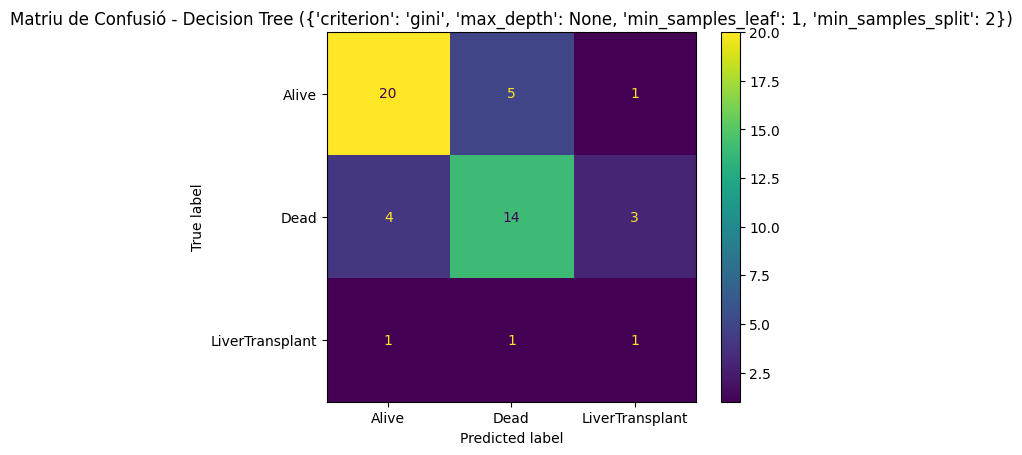
\includegraphics[width=0.95\linewidth]{img/dt-cm.png}
	\caption{Matriu de confusió de les prediccions de l'Arbre de Decisió (amb paràmetres \textit{criterion = `gini', max\_depth = None, min\_samples\_leaf = 1} i \textit{min\_samples\_split = 2}) en el conjunt de test.}
	\label{fig:dt-cm}	
\end{figure}

En aquest model, la classe `Alive' s'ha predit correctament en una proporció de $\dfrac{20}{26} \approx 0,7692$ i en la classe `Dead' $\dfrac{14}{21} \approx 0,6667$. Aquests resultats són pitjors que pel KNN i en aquest cas el model és millor predint la classe majoritària (`Alive'). Com ja hem dit, la part positiva d'aquest model és que ha aconseguir predir correctament una de les tres mostres de `LiverTransplant'; però, com que hi ha molt poques mostres, s'ha de tenir menys en compte aquesta classe.

%--------------------------------------------------------------------------
\subsection{Support Vector Machine (SVM)}

\subsubsection{Motivació}
Les SVM ofereixen una gran flexibilitat mitjançant l'ús de diferents funcions de kernel. Això ens permet explorar diferents maneres de modelar les relacions no lineals entre les variables i la variable objectiu "Status". Per exemple, un kernel polinòmic o de base radial (RBF) pot capturar relacions complexes que podrien ser crucials per la nostra predicció.

Un altre avantatge important de les SVM és la seva capacitat de controlar l'equilibri entre l'error de classificació i la complexitat del model a través del paràmetre de regularització C. Això és especialment útil quan es treballa amb dades mèdiques, on el balanç entre sensibilitat i especificitat és fonamental.

Finalment, la robustesa de les SVM davant dades amb soroll o outliers les fa una opció atractiva per a datasets complexos i desordenats com pot ser el nostre.

\subsubsection{Mètriques}
De la mateixa manera que s'ha fet per al KNN i per a l'Arbre de Decisió, en l'avaluació del model s'ha utilitzat la mètrica de \textit{f1-score-weighted}. Aquesta mètrica és calcula fent la mitjana harmònica entre la \textit{precision} i el \textit{recall}, penalitzant els valors extrems (calen valors bons tant de \textit{precision} com de \textit{recall} per tal de tenir un bon \textit{f1}). La mitjana de valors de totes les prediccions es fa ponderada (\textit{weighted}), de manera que a cada classe se li dona una importància proporcional a les seves aparicions. D'aquesta manera, es puntua millor que s'aconsegueixi classificar correctament la classe majoritària (on s'haurà de fer més prediccions). 

Si en un altre experiment es desitgés predir donar molta importància la classe minoritària (en aquest cas ``LiverTransplant'', que no és tant rellevant en aquest estudi com ``Alive'' o ``Dead'') es podrien utilitzar altres mètriques que ho tinguessin més en consideració.

\subsubsection{Hiperparàmetres}
Pel que fa als hiperparàmetres de la SVM, s'han modificat el kernel, el paràmetre C i el paràmetre gamma.

Els valors que es provaran per cada un dels paràmetres són els següents:
\begin{itemize}
	\item \textbf{Kernel}: `linear', `poly', `sigmoid', `rbf'.
	\item \textbf{C}: 0.1, 0.5, 1, 2, 3, 5.
	\item \textbf{Gamma}: `scale', `auto'.
\end{itemize}

El significat de cada paràmetre és el següent:
\begin{itemize}
	\item \textbf{Kernel}: aquest paràmetre representa la funció matemàtica que s'utilitzarà per transformar les dades a un espai de major dimensionalitat i així poder trobar relacions no lineals per separar les dades per un hiperplà. 
	\begin{itemize}
		\item `linear': aquest kernel no fa cap transformació, sinó que manté les dades en el seu espai original. És simple i computacionalment més barat.
		\item `poly': aquest kernel transforma les dades a un espai de major dimensió on les combinacions polinòmiques dels atributs originals esdevenen les noves dimensions. Permet modelar interaccions més complexes entre variables que el kernel lineal. El seu comportament depèn d'un paràmetre `degree' que controla el grau polinòmic. En el nostre cas, s'ha deixat sempre el grau per defecte, que és 3.
		\item `sigmoid': aquest kernel utilitza una funció sigmoide (semblant a la funció d'activació en xarxes neuronals). És capaç de transformar l'espai de dades de maneres no lineals i no polinòmiques.
		\item `rbf': aquest és un dels kernels més populars en les SVM. Transforma les dades a un espai on la distància radial (basada en la distància euclidiana) des d'un punt central determina el valor de cada nova dimensió. És molt efectiu per capturar relacions complexes en les dades i depèn del paràmetre gamma, que controla l'amplitud de la `zona d'influència' de cada un dels punts de suport.
	\end{itemize}	
	
	\item \textbf{C}: aquest paràmetre controla l'equilibri entre la maximització del marge i la minimització de l'error en la classificació. Un valor més alt penalitza més els errors i disminueix el marge (pot portar a overfitting); mentre que un valor més baix permet més errors i augmenta el marge (pot portar a underfitting).
	
	\item \textbf{Gamma}: aquest paràmetre és per el kernel `rbf' i controla si es té en compte una àrea més o menys gran per cada punt de suport a l'hora de determinar el límit de decisió.
	\begin{itemize}
		\item `scale': amb aquest paràmetre, la gamma s'adapta automàticament a l'escala de les dades. Ajuda a prevenir que el model sigui massa sensible a les variacions el les dades quan hi ha moltes dimensions o quan les característiques tenen variàncies molt diferents.
		\item `auto': aquest enfoc no té en compte la variància de les dades i pot no ser tant òptim som `scale' en certs casos.
	\end{itemize}		
\end{itemize}

Totes les possibles combinacions d'aquests paràmetres es provaran mitjançant  Grid Search i cross validation per trobar els que millor rendiment aporten al model.

\subsubsection{Millor conjunt de dades}
Per trobar el conjunt de dades que proporciona un millor rendiment a aquest model, s'han fixat els següents hiperparàmetres:
\begin{itemize}
	\item \textbf{Kernel}: `rbf'.
	\item \textbf{C}: 1.
	\item \textbf{Gamma}: 'scale'.
\end{itemize}

Amb aquests paràmetres fixats, s'ha executat la funció \texttt{find\_best\_dataset()}. Després que es provin totes les combinacions possibles de modificacions al dataset inicial (un total de 64 combinacions), la que ha obtingut millors resultats de \textit{f1-score-weighted} en el test és la següent:
\begin{itemize}
	\item No eliminar outliers.
	\item Eliminar les files amb més de 9 NaNs.
	\item Escalar les variables numèriques amb \textit{MinMax}.
	\item Imputar variables numèriques amb KNN Imputer (amb $k = 15$) i les categòriques amb Random Forest Classifier (amb el criteri `gini'). Els resultats de la imputació (calculats tal i com s'ha explicat en l'apartat \ref{subsec:missings}) han estat de 0,3808 de mitjana entre la puntuació $R^2$ de les numèriques i \textit{f1-score-weighted} de les categòriques.
	\item Codificar les variables categòriques amb \textit{Ordinal Encoding}.
	\item Balancejar les classes de la variabe objectiu mitjançant \textit{SMOTE}.
\end{itemize}

Amb aquestes modificacions i els paràmetres fixes que s'han mencionat, s'ha aconseguit un resultat de 0,8201 de \textit{f1-score-weighted} en el conjunt de prova, que es pot considerar un resultat bastant bo. La partició de train conté 441 mostres i la de test 50. A partir d'aquí s'ha considerat que aquests són els millors conjunts de dades per els models d'Arbre de Decisió, i el següent pas serà trobar els millors paràmetres per el model en aquest dataset.

\subsubsection{Millors hiperparàmetres pel dataset escollit}
Una vegada determinat el millor dataset per els models de SVM, cal provar quins són els millors paràmetres. Això es fa mitjançant la funció \texttt{run\_experiment()} que cridarà a \texttt{svm\_prediction()}. En aquesta segona funció s'implementa cross validation amb 5 \textit{folds} per cada possible combinació de paràmetres. Una vegada s'hagin provat tots els paràmetres, la combinació de paràmetres que tingui un millor \textit{f1-score-weighted} de mitjana en la partició de validació (és a dir, el que obtingui una millor puntuació en la validació creuada) es determinarà com la millor per el model de SVM i s'executarà la predicció en el test.

Una vagada s'ha fet la l'execució, s'ha obtingut que la millor combinació de paràmetres és la següent:
\begin{itemize}
	\item \textbf{Kernel}: `linear'.
	\item \textbf{C}: 100.
	\item \textbf{Gamma}: 'scale'.
\end{itemize}

Amb aquests paràmetres s'ha obtingut una puntuació en la partició de validació de 0,7463. Cal mencionar que el paràmetre gamma no és rellevant en un kernel linear, així que no s'ha de considerar que afecti al model.

\subsubsection{Resultats}
Amb el dataset escollit i els millors hiperparàmetres triats, la predicció en el conjunt ha obtingut les mètriques que es poden veure en la taula \ref{tab:svm-test}

\begin{table}[H]
\centering
\begin{tabular}{l|l}
\hline
\textbf{Metric} & \textbf{Value} \\
\hline
accuracy & 0.8 \\
f1-micro & 0.80000000000000002 \\
f1-macro & 0.7362502681006221 \\
f1-weighted & 0.8139203970953212 \\
precision-micro & 0.8 \\
precision-macro & 0.7143939393939394 \\
precision-weighted & 0.8601363636363637 \\
recall-micro & 0.8 \\
recall-macro & 0.8626373626373626 \\
recall-weighted & 0.8 \\
\hline
\end{tabular}
\caption{Mètriques de les prediccions del Support Vector Machine (amb paràmetres \textit{C = 5, gamma = `scale'} i \textit{kernel = `linear')} en el conjunt de test.}
\label{tab:svm-test}
\end{table}

Si ens fixem en la mètrica que hem escollit (\textit{f1-score-weighted}), podem veure que s'ha obtingut un valor de 0,8139, que és un valor molt bo, inclús lleugerament més alt del que s'ha vist en el cross validation. Això pot ser degut a factors aleatoris.

Pel que fa a les prediccions, en la figura \ref{fig:svm-cm} es pot veure la matriu de confusió d'aquest model en les prediccions del conjunt de test. La majoria de prediccions són bones, però hi ha hagut 7 mostres `Alive' que no s'han predit correctament, 3 de `Dead'. En aquest model, la classe `LiverTransplant' s'ha predit bé el 100\% de les vegades (tot i només haver-hi 3 mostres), a més d'haver valors de `Alive' i de `Dead' que s'han predit erròniament com a `LiverTransplant'. Observant això, podem dir que aquest model té una major tendència a predir la classe `LiverTransplant' en comparació als dos models previs.

\begin{figure}[H]
	\centering
	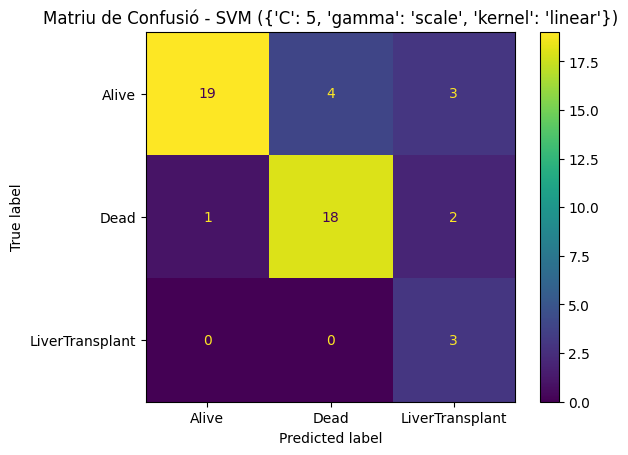
\includegraphics[width=0.85\linewidth]{img/svm-cm.png}
	\caption{Matriu de confusió de les prediccions del Support Vector Machine (amb paràmetres \textit{C = 5, gamma = `scale'} i \textit{kernel = `linear')} en el conjunt de test.}
	\label{fig:svm-cm}	
\end{figure}

En aquest model, la classe `Alive' s'ha predit correctament en una proporció de $\dfrac{19}{26} \approx 0,7308$ i en la classe `Dead' $\dfrac{18}{21} \approx 0,8571$. Aquests resultats són més semblants al KNN que no pas a l'Arbre de Decisió. no obstant la sorpresa, com ja s'ha dit, és que s'han predit correctament tots els valors de `LiverTransplant'.

Es pot dir que, en aquest model SVM, no hi ha pràcticament tendència a predir arbitràriament la classe majoritària perquè la majoria de falsos positius es troben quan es predeia `LiverTransplant' o `Dead' (classes minoritàries en comparació amb `Alive'), a més de que són les classes on hi ha més percentatge de prediccions correctes.

%--------------------------------------------------------------------------


